% Physics experiment report
% 30/Sep/2016

\documentclass[a4paper,10pt,notitlepage]{report}

\usepackage{CJKutf8}
\usepackage{amsmath}
\usepackage{indentfirst}
\usepackage{graphicx}

\setlength{\parindent}{2em} 

\begin{CJK*}{UTF8}{gbsn}
\begin{document}

\title{测定冰的熔化热实验报告}
\author{秦光辉\ 9组3号}
\maketitle

\section*{一、实验数据处理}

	表一所示的数据是实验中一些可以直接观测和见解获得的数据,$m_0$是桶和搅拌器的质量,$m_i$是开始的时候水、桶、搅拌器的质量,$m_f$是冰融化以后水、桶、搅拌器的质量,$T_i$是冰的质量,$T_e$是环境温度。
	
\begin{table}[htbp]
\centering
	\begin{tabular}{|l|l|l|l|l|l|l|}
	
		\hline
		$m_0$/g & $m_i$/g & $m_f$/g & $m_{water}$/g & $m_{ice}$/g & $T_i$/$^{\circ}$C & $T_e$/$^{\circ}$C \\
		\hline
		144.19 & 326.53 & 353.99 & 182.34 & 27.46 & -17.3 & 26.0 \\
		\hline
		\multicolumn{7}{c}{\scriptsize Table 1\ 影响时间结果的一些物理量测量数据表} \\

	\end{tabular}
\end{table}

	以下是温度随时间的变化数据表
	
\begin{table}[htbp]
\centering
	\begin{tabular}{|l|l|l|l|l|l|l|l|l|l|l|l|l|}
	
		\hline
		t/s & 0 & 15 & 30 & 45 & 60 & 75 & 120 & 125 & 130 & 135 & 140 & 145 \\
		\hline
		T/$^{\circ}$C & 37.0 & 37.0 & 37.0 & 36.9 & 36.9 & 36.9 & 35.4 & 35.0 & 34.7 & 34.1 & 33.1 & 32.4 \\
		\hline
		\hline
		t/s & 150 & 155 & 160 & 165 & 170 & 175 & 180 & 185 & 190 & 195 & 200 & 205 \\
		\hline
		T/$^{\circ}$C & 31.1 & 30.0 & 28.4 & 27.1 & 26.1 & 25.3 & 24.5 & 24.0 & 23.6 & 23.2 & 22.9 & 22.7 \\
		\hline
		\hline
		t/s & 210 & 215 & 220 & 225 & 230 & 235 & 240 & 245 & 250 & 255 & 260 & 265 \\
		\hline
		T/$^{\circ}$C & 22.4 & 22.3 & 22.1 & 22.0 & 22.0 & 22.0 & 22.0 & 22.0 & 22.0 & 22.0 & 22.0 & 22.1 \\
		\hline
		\multicolumn{13}{c}{\scriptsize Table 2\ 温度随时间变化数据表} \\

	\end{tabular}
\end{table}

	将上述数据绘制成散点图一,可以看出温度随着时间先迅速下降,然后逐渐平缓,最后略有回升。虽然水处于一个相对绝热的环境中,但是水温依然会越来越接近于室温,可见我们的绝热装置并不十分理想,所以我们的实验补偿是必不可少的。在末态的时候水温回升的速率没有刚开始下降得快,因为末态的时候水温和室温相对接近,温差不大。 \\
	
\begin{figure}[htbp]
\centering

	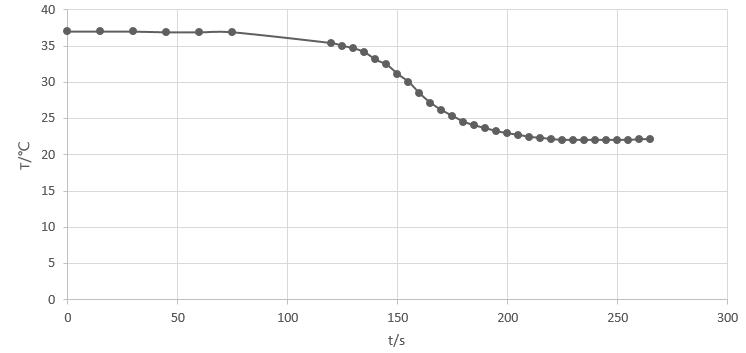
\includegraphics[scale=.6]{1.jpg}
	\begin{center}
		\scriptsize Figure 1 T-t散点图
	\end{center}

\end{figure}
	
	取水的温度为$T_2 = 36.8 ^{\circ}$C,末态平衡温度为$T_3 = 22.0^{\circ}$C,可以计算得冰的熔化热为:
	
\begin{align*}
	L = \frac{(m_0 * c_{copper} + m_{ice} * c_{water})(T_2 - T_3)}{m_{ice}} - c_{water}(T_3 - T_i) \\
	- c_{ice}(T_i - T_1) = 3.23 * 10^5 J/kg
\end{align*}

\section*{二、分析和讨论}
\subsection*{1.误差来源分析}
	
	我在第一次做实验的时候,由于我没有控制好初始水温,冰熔化之后并没有降到室温以下,实验数据见表三。
	
\begin{table}[htbp]
\centering
	\begin{tabular}{|l|l|l|l|l|l|l|l|l|l|l|l|l|}
	
		\hline
		t/s & 0 & 15 & 30 & 45 & 60 & 75 & 105 & 110 & 130 & 135 & 140 & 145 \\
		\hline
		T/$^{\circ}$C & 38.5 & 38.5 & 38.4 & 38.4 & 38.3 & 37.8 & 37.3 & 37.1 & 36.6 & 35.5 & 35.0 & 34.3 \\
		\hline
		\hline
		t/s & 150 & 155 & 160 & 165 & 170 & 175 & 180 & 185 & 190 & 195 & 200 & 205 \\
		\hline
		T/$^{\circ}$C & 33.8 & 37.3 & 32.9 & 32.5 & 32.2 & 31.9 & 31.6 & 31.4 & 31.2 & 31.0 & 30.8 & 30.6 \\
		\hline
		\hline
		t/s & 210 & 215 & 220 & 225 & 230 & 235 & 240 & 245 & 250 & 255 & 260 & 265 \\
		\hline
		T/$^{\circ}$C & 30/4 & 30.2 & 30.1 & 30.0 & 29.9 & 29.8 & 29.7 & 29.6 & 29.6 & 29.5 & 29.5 & 29.5 \\
		\hline
		\multicolumn{13}{c}{\scriptsize Table 3\ 附加实验数据表} \\
		
	\end{tabular}
\end{table}

		当时水+桶的质量为288.05g,水+冰+桶的质量为302.27g,可以计算得冰的熔化热为
		
\begin{equation*}
	L = 3.44 * 10^5 J/kg
\end{equation*}

	可见温度补偿并不会对实验产生决定性影响,我认为实验的主要的误差来源是冰的质量测量。在投放冰块的时候往往容易飞溅出水滴,在搅拌中容易用力过大而使得水滴落到杯盖上,这样会使冰的质量测量值偏低。冰的质量本身就很小,这样一来相对误差就非常之大。 \\
	
\subsection*{2.补偿法}

	物理实验中往往会面对很多无法确定的干扰,这些干扰无法避免,影响我们的实验。这些影响往往难以量化描述,无法确切地反映在实验数据中,我们只能用补偿法尽可能地规避这些因素对我们实验的影响。比如在这次实验中,我们使用了热交换补偿。补偿之后我们仍然不知道数据的偏差具体是多少,但是我们却可以减小它的影响! \\
	
\subsection*{3.数据偏小的原因}

\begin{enumerate}
	
	\item 实验中取冰块往往花费很长时间,冰块熔化,有水分残留在冰块表面
	\item 温度计的热容未考虑在内
	\item 冰块用制冰机制作,冷冻时间不够长,而且可能含有杂质或者气泡等,这些都对实验数据产生影响	
	
\end{enumerate}

\section*{三、感悟和收获}

	测定冰的熔化热是一个很有意思的实验,但是也是一个很考验能力的实验。我一直都不是一个很灵巧的人,实验中不是忘了搅拌就是忘了记录水的质量,或者是投放冰块的时候水滴飞溅,最后L变得非常大。我一连做了四次才成功,这是对我的一次锻炼。物理不仅仅有理论计算,也有很多实验。我不应该忘记物理是一门实验科学,而实验只有多训练才能有进步,我应该吸取这次教训,以后更加努力! \\

\end{CJK*}
\end{document}
